\documentclass[a4paper]{article}

\def\npart {IB}
\def\nterm {Michaelmas}
\def\nyear {2017}
\def\nlecturer {J.M.Evans (j.m.evans@damtp.cam.ac.uk)}
\def\ncourse {Quantum Mechanics}

\include{header}

\begin{document}
\maketitle

\setcounter{section}{-1}
\section{Introduction}




Quantum Mechanics (QM) is a radical generalization of classical physics involving a new fundamental constant, \emph{Planck's constant}:

\[ \hbar = h / 2\pi \approx 1.05 \times 10^{-34} \text{Js},
 \]
 

 
 with dimensions 
 
 \begin{align*}
 [\hbar] = ML^{2} T^{-1} & =  \text{[position]} \times \text{[momentum]} \\
 & =  \text{[energy]} \times \text{[time]}
 \end{align*}
 
 Profound new features of QM include:
 
 \begin{itemize}
 	\item \emph{ Quantisation.} Physical quantities such as energy may be restricted to discrete sets of values, or may appear only in specific amounts, called \emph{quanta}.
 	
 	\item \emph{Wave-particle duality}. Classical concepts of a particle and a wave are merged; they become different aspects of a single entity that shows either particle-like or wave-like behaviour, depending on the circumstance.
 	
 	\item \emph{Probability and uncertainty}. Predictions in QM involve probability in a fundamental way and there are limits to what can be asked about a physical system, even in principle\footnote{If we were able to keep track of every single particle we would know exactly what the system is doing. But in QM, we \emph{still} can't know what the system is doing precisely. }. A famous example is the \emph{Heisenberg uncertainty principle relation} for position and momentum. 
\end{itemize}

Despite these radical changes, classical physics must be recovered in the limit $ \hbar \to 0 $ (which may require careful interpretation).


The following sections provide some physical background and summarise key experimental evidence for these novel features of QM.
 
\subsection{Light Quanta}

An electromagnetic (EM) wave, eg. light, consists of quanta called \emph{photons}. Photons can be regarded as particles with energy, $ E $, and momentum, $ p $, related to frequency $ \nu $ or $ \omega $, and\footnote{$ v,\omega $  both called frequency, and differ by a factor of $ 2 \pi $.} wavelength $ \lambda $, or wavenumber $ k $, according to

\[ E = h v = \hbar \omega \]
\[ p = h / \lambda = \hbar k \]

  


From the wave equation (satisfied by each EM field component) 

\[ c = \omega / k  = v k \quad \text{ or } \quad E = cp \text{ massless particle}\]

so the relations are consistent with photons being particles of rest mass zero, moving with the speed of light, $ c $.

Compelling evidence for the existence of photons is provided by the \emph{photoelectric effect}. Consider (Fig. 1) light of EM radiation $ (\gamma) $ of frequency $ \omega $ incident on a metal surface. For certain metals and suitable frequencies this results in the emission of electrons $ (e^{-}) $ and their maximum kinetic energy $ K $ can be measured. 


\begin{center}
	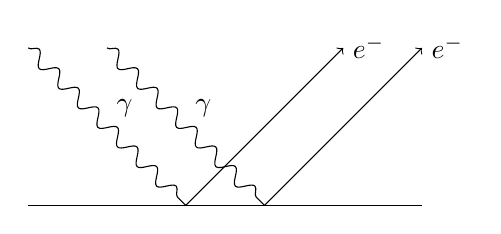
\begin{tikzpicture}
	\draw (-2, 0) -- (3, 0);
	\draw [decorate, decoration={snake}] (-2, 2) -- (0, 0) node [pos = 0.5, anchor=south west] {$\gamma$};
	\draw [decorate, decoration={snake}] (-1, 2) -- (1, 0) node [pos = 0.5, anchor=south west] {$\gamma$};
	\draw [->] (0, 0) -- (2, 2) node [right] {$e^{-}$};
	\draw [->] (1, 0) -- (3, 2) node [right] {$e^{-}$};
	\end{tikzpicture}
\end{center}


Experiments find that:

 \begin{enumerate}
 	\item the rate at which electrons are emitted is proportional to the intensity of the radiation (the `brightness' of the source); 
 	\item $ K $ depends linearly on $ \omega $ but \emph{not} on the intensity; 
 	\item for $ \omega < \omega_{0} $, some critical value, \emph{no} electrons are emitted, irrespective of the intensity. 
 	
 \end{enumerate}

The results are extremely hard to understand in terms of classical EM waves. However, they follow naturally from the assumption that the wave consists of photons, each with energy $ E = \hbar \omega $, and with the intensity of the radiation proportional to the number of photons incident per unit time. Suppose that an electron is emitted as a result of absorbing a single photon with sufficiently high energy. If $ W $ is the minimum energy needed to liberate an electron from the metal then

\[ K = \hbar \omega - W \]

is the maximum kinetic energy of an emitted electron if $ \omega > \omega_{0} $, where $ \omega_{0}  = W / \hbar $, and no emission is possible if $ \omega < \omega_{0} $ (Fig 2). Furthermore, the rate at which electrons are emitted will be proportional to the rate at which incident photons arrive, and hence the intensity.

\begin{center}
	\begin{tikzpicture}
	\draw [-> ](-0.5, 0) -- (5, 0) node [right] {$ \omega $};
	\draw [->] (0, 0) -- (0, 3) node [above] {$ K $};
	\draw (1, 0) node [below] {$w_{0} = \frac{w}{\hbar}$} -- (4, 2) ;
	\end{tikzpicture}
\end{center}






The energy-frequency relation for photons was introduced by Planck and used to derive the \emph{black body spectrum}. This is the distribution of energy with frequency for EM radiation in thermal equilibrium, a fundamental result in thermodynamics of far-reaching importance (understanding the \emph{cosmic microwave background}, for example). Einstein then applied the energy-frequency relation to explain the photoelectric effect. Further conclusive evidence for photons as particles, including the momentum-wavelength relation, came from subsequent experiments involving \emph{Compton scattering. }

Consider a photon of wavelength $ \lambda $ colliding with an electron that is stationary in the laboratory frame. Let $ \lambda' $ be the wavelength of the photon after the collision and $ \theta $ the angle through which it is deflected. Treating the photon as a massless relativistic particle, conservation of four-momentum implies

\[ \lambda' - \lambda = \frac{h}{m_{e}c} (1 - cos \theta) \] 

\begin{center}
	\begin{tikzpicture}
	\draw ;
	\draw [decorate, decoration={snake}] (-3, 0) -- (1, 0) node [pos = 0.5, anchor=south west] {$\gamma(\lambda)$};
	\draw [decorate, decoration={snake}] (1, 0) -- (3, 2) node [pos = 0.5, anchor=south east] {$\gamma$};
	\draw [->] (1, 0) node [below] {$e^{-}$} -- (3, -2) node [right] {$e^{-}$};
	\draw [dashed] (1,0) -- (3,0);
	\draw (1.5, 0) arc (0:65:0.4);
	\draw node at (1.35,0.35) [below] {$ \theta $}; 
	\end{tikzpicture}
\end{center}

This dependence of the change in wavelength (or decrease in energy) can be verified experimentally (for $ X $-rays, or $ \gamma $-rays, for instance). 

\subsection{Bohr Model of the Atom}

The \emph{Rutherford model} of the atom was proposed to explain the results of scattering experiments (eg. alpha particles scattered by gold foil). The key assumption is that most of the mass of the atom is concentrated in a compact, positively-charged \emph{nucleus} (subsequently understood to consist of protons and neutrons), with light, negatively charged electrons orbiting around it. The simplest case is the Hydrogen atom, in which a single electron with charge $ - e $ and mass $ m_{e} $ orbits a nucleus consisting of a single proton with charge $ +e $ and mass $ m_{p} $. Since $ m_{p} >> m_{e} $ it is a good approximation to assume the proton is stationary, at the origin, say. The electron and proton interact via Coulomb's Law: the potential energy of the electron and the force it experiences are:
\[ V(r) = - \frac{e^{2}}{4\pi \varepsilon_{0}} \frac{1}{r} \qquad \mathbf{F}(\mathbf{r}) =  - \nabla V = - \frac{e^{2}}{4\pi \varepsilon_{0}} \hat{\mathbf{r}}\]

The classic equations of motion for the electron imply that its angular momentum, $ \mathbf{L} = \mathbf{r} \times \mathbf{p} $, and its total energy,

\[ E = \frac{1}{2} m_{e} v^{2} - \frac{e^{2}}{4 \pi \varepsilon_{0}} \frac{1}{r}  \]

are constant. The orbits are therefore planar and they can be determined exactly. For any value of $ E < 0 $ there is a closed orbit and the electron is \emph{bound} to the proton to form a Hydrogen atom. For orbits with $ E > 0 $ the electron eventually escapes to infinity: it is not bound to the proton.

Despite its success in accounting for Rutherford scattering, this model has a number of problems. The treatment is identical, mathematically, to planetary orbits governed by gravity (see Part IA Dynamics and Relativity, for example) but an important additional feature of electromagnetism has been left out. An accelerating charge radiates energy (carried away via EM fields) and this means that the electron would actually spiral inwards towards the proton: this is not a good model of a stable atom!


There is also experimental evidence for complex discrete structure within atoms. This comes from \emph{line spectra}: bright emission lines (from a hot sample) or dark absorption lines (if radiation is passed through a cooler sample), both occurring at certain characteristic wavelengths or frequencies. This suggests that an atom can emit or absorb radiation only at these particular frequencies or wavelengths, which corresponds to photon with particular energies.

The \emph{Bohr model} restricts the classical orbits of the Rutherford model by postulating that the angular momentum of the electron obeys the \emph{Bohr quantisation condition}

\[ L = n \hbar, \qquad n = 1,2,\cdots,\]
 
with only these discrete values are allowed. This might seem to be an unsatisfactory way to address the issue of stability, but it proves to be remarkably successful in reproducing the complex experimental data relating to line spectra.

Specializing to circular orbits (Fig. 4) for simplicity, we have 

\[ F = m_{e} v^{2} / r \qquad \text{ and } \qquad L = m_{e} r v \]

 \begin{center}
	\begin{tikzpicture}
	\draw [ ->] (2, 0) node [right] { $ m_{e} $ } -- (2, 2) node [right] {$ v $};
	\draw [->] (0, 0) node [below] {$ m_{p} $}  -- (2, 0) node [pos = 0.5, below] {$r$};
	\draw [->-=0.1] (0, 0) circle [x radius = 2, y radius = 2];
	\end{tikzpicture}
\end{center}

It is then straightforward to check that the quantisation condition leads to the following set of \emph{Bohr orbits}

\[ r_{n} = \frac{4 \pi \varepsilon_{0} \hbar^{2}}{m_{e} e^{2}} n^{2}, \quad v_{n} = \frac{e^{2}}{4 \pi \varepsilon_{0} \hbar} \frac{1}{n}, \quad E_{n} 
= - \frac{1}{2} m_{e} \left(  \frac{e^{2}}{4 \pi \varepsilon_{0} \hbar} \right)^{2} \frac{1}{n^{2}}, \quad n = 1,2,\cdots   \]

Note that the allowed energy levels are now discrete. 

Suppose that an electron makes a transition between levels $ n $ and $ n' $ (with $ n' > n $, say) accompanied by emission or absorption of a photon of frequency $ \omega $ (Fig 5). Then

\[ \hbar \omega = E_{n'} - E_{n} = \frac{1}{2}m\left( \frac{e^{2}}{4 \pi \varepsilon_{0} \hbar }^{2} \right)^{2} \left( \frac{1}{n^{2}} - \frac{1}{n'^{2}} \right)   \]
 

\begin{center}
	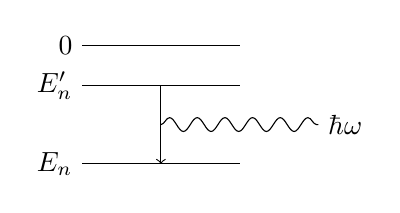
\begin{tikzpicture}
	\draw (-1, 0) node [left] {$0$} -- (1, 0);
	\draw (-1, -0.5) node [left] {$E_n'$} -- (1, -0.5);
	\draw (-1, -1.5) node [left] {$E_n$} -- (1, -1.5);
	\draw [->] (0, -0.5) -- (0, -1.5);
	\draw [decorate, decoration={snake}] (0, -1) -- (2, -1) node [right] {$\hbar \omega$};
	\end{tikzpicture}
\end{center}

This formula accounts for a vast amount of experimental data on spectral lines for Hydrogen. The Bohr model also provides an estimate for the \emph{size} of the Hydrogen atom $ r_{1} \approx 5.29 \times 10^{-11} \text{m} $, the \emph{Bohr radius}. Despite these considerable successes, the origin of the Bohr quantisation condition seems obscure. A better explanation is needed.

\subsection{Matter Waves}

The relations used to associate particle properties ($ E $ and $ p $) to waves can also be used to associate wave properties ($ v $ or $ omega $ and $ \lambda $ or $ k $) to particles. This applies not just to relativistic photons but also to non-relativistic particles, electrons for example, and $ \lambda $ is called the \emph{de Broglie wavelength} of the particle. A strong hint that this might be important for a better understanding of the Bohr quantisation condition comes from observing that for a circular orbit

\[ L = pr = n \hbar \quad \iff \quad n \lambda = 2 \pi r \]

The Bohr condition therefore says that the circumference of each orbit is exactly an integral number of de Broglie wavelengths. 

[Fig 6]

It can also be verified experimentally that electrons do indeed exhibit wave-like behaviour, and a helpful idealisation is the \emph{double slit experiment}. Consider a source which emits a beam of electrons, a barrier with two slits that can be open or closed, and a screen on which the electrons are detected. 

Suppose that first one slit is open and the other is closed. We cannot say with certainty where any particular electron will be detected, but after many electrons have been emitted, the number detected varies with tranverse position. If \emph{both} slits are open, however, then the electrons produce (perhaps unexpectedly) an interference pattern.

\begin{center}
	\begin{tikzpicture}
	\draw (4, -2) -- (4, 2);
	
	\foreach \x in {-1, -2, -3} {
		\draw (\x, -2) -- (\x, 2);
	}
	
	\draw [<->] (-2, -1.7) -- (-3, -1.7) node [below, pos=0.5] {$\lambda$};
	\draw [->] (-3, 2.3) -- (-1.5, 2.3) node [right] {wave};
	
	\draw (0, 0.55) -- (4, 1.5);
	\draw (0, -0.55) -- (4, 1.5);
	\draw [domain=-2:2,samples=50, mblue] plot [smooth] ({4 + 1.5 * exp(-\x * \x) * (cos (200 * \x))^2}, \x);
	\draw [->, align=left] (4, 0) -- (6, 0) node [right] {density of\\ electrons};
	
	\draw [dashed] (0, 0.55) -- (0.34, -0.375);
	\node at (0.20, -0.45) [below] {$\delta$};
	
	\draw [mred, fill=white] (-0.05, -0.5) rectangle (0.05, 0.5);
	\draw [mred, fill=white] (-0.05, 0.6) rectangle (0.05, 2);
	\draw [mred, fill=white] (-0.05, -0.6) rectangle (0.05, -2);
	\end{tikzpicture}
\end{center}

This matches the interference pattern obtained for waves of length $ \lambda $ incident on a barrier. Consider a point $ P $ at some fixed perpendicular distance from the barrier, and let $ \delta $ be the difference of the distances to $ P $ from each of the slits. Constructive interference occurs for $ \delta = n \lambda $ while destructive interference occurs for $ \delta = (n + 1/2)\lambda $. The result is that the (amplitude)$^{2}$ of the superposed waves varies as $ P $ varies.

In diffraction experiments with electrons, we cannot predict what will happen to any \emph{single} particle; the most that can be said is that it will be detected at a given position with a certain \emph{probability}. The diffraction pattern is conclusive evidence of interference and so confirms the existence of matter waves, and diffraction experiments allow an experimental determination of the de Broglie wavelength. The results also suggest that the probability distribution for particles can be expressed as the (amplitude)$^{2}$ of a wave. 
 



\section{Wave functions and Operators}

In first few chapters we consider a quantum particle in one dimension, introduce some key ideas and three postulates for how to extract physical information from mathematical framework. Later (Chapter 6) we will state general axioms from which these follow. 

\subsection{Wave functions and States  }

A classical point particle in one-dimension has a position $ x $ at each time. In QM a particle has a \emph{state} at each time given by a complex-valued, \footnote{non-zero} wavefunction 

\[ \psi(x) \]

Postulate(P1): A measurement of position gives a result with probability density $ | \psi(x) |^{2} $. ie. $ | \psi(x) |^{2} \delta x $ prob particle is found between $ x $ and $ x + \delta x $, or 

\[ \int_{a}^{b} | \psi(x) |^{2} \; \d x \]

is the probability the particle is found in the interval $ a \leq x \leq b $.
This requires $ \psi(x) $ is \emph{normalised}.

\[ \int_{-\infty}^{\infty} | \psi(x) |^{2} \; \d x = 1 \qquad \text{ single particle - total probability 1 } \]

\begin{eg}(Gaussian wavefunction)
	
	\[ \psi(x) = C e^{- (x - x_{0})^{2} / 2 \alpha } \qquad \text{ real } \alpha > 0 \]
	
	
	 \begin{center}
	 	%label axis x,y as x, |psi(x)|^{2}
		\begin{tikzpicture}[yscale=1.5]
		\draw [->] (-3, 0) -- (3, 0) node [right] {$x$};
		\draw [->](0, 0) node [below] {$x_{0}$}  -- (0, 1.3) node [above] {$| \psi(x) |^{2}$};
		\draw [domain=-3:3,samples=50, mblue] plot (\x, {exp(-\x * \x)});
		\end{tikzpicture}
	\end{center}



\begin{align*}
	\int_{-\infty}^{\infty} | \psi(x) |^{2} \; \d x & = | C |^{2} \int_{- \infty}^{\infty} e ^{ - (x - x_{0})^{2} / \alpha} \; \d x \\
	& = | C |^{2} (\alpha \pi)^{\frac{1}{2}} = 1
\end{align*}

So \footnote{Recall $ \int_{-\infty}^{\infty}  e^{-\frac{(x-\mu)^{2}}{2 \sigma^{2}}} \; \d x = \sqrt{2\pi \sigma^{2}}  $}   $ \psi $ normalised if $ C = \left( \frac{1}{\alpha \pi} \right)^{\frac{1}{4}}  $.
$ \alpha $ small $ \Rightarrow $ sharp peak around $ x = x_{0} $, $ \Rightarrow $ ``particle-like".
$ \alpha $ large $ \Rightarrow $ more spread out (diffuse)
 
\end{eg}

It is convenient to deal more generally with \emph{normalisable} wavefunctios

\[ \int_{-\infty}^{\infty} | \psi(x) |^{2} \; \d x < \infty \qquad \text{ finite/convergent} \]
   
Then $ \psi(x) $ and   $  \phi(x) = \lambda \psi(x) $ are physically equivalent and represent same state for any $ \lambda \neq 0 $. Provided $ \psi $ normalisable, we can choose $ \lambda $ so that $ \phi $ normalised. But if $ \psi $ normalised already, then $ \phi(x) = e^{i \alpha} \psi(x) $ (for any real $ \alpha $) gives some probability distribution. 

\[ | \phi(x) |^{2} = | \psi(x) |^{2} \]

So quantum state is strictly an equivalence class of non-zero wave functions but in practice we often refer to $ \psi(x) $ as ``the state''.

Any non-zero normalisable wave function $ \phi(x) $ represents a physical state. For our purposes we can assume, \emph{unless} we say otherwise, $ \psi(x) $ is smooth (can be differentiated any number of times), and $ \psi(x) \to 0 $ as $ | x | \to \infty $

If $ \psi_{1}(x) $ and $ \psi_{2}(x) $ are normalisable then so is 

\[ \psi = \lambda_{1} \psi_{1} + \lambda_{2} \psi_{2} \] 

for any complex $ \lambda_{1},\lambda_{2} $.

Physically: principle of super position
Mathematically: structure of complex vector space.

\begin{eg} (Superposition of Gaussians)
	\[ \psi(x) = B( e^{\frac{-x^{2}}{2\alpha}}  + e^{-(x-x_{0})^{2}/2\beta}) \]
	
	Can choose $ B $ so that $ \psi $ is normalised
	
	
	 \begin{center}
	 	% \draw [ ->](0, 0) -- (0,1.3) node[above] {$| \psi(x) |^{2}$
	 	%dashed vertical line going through the second wave, label with x_{0}
		\begin{tikzpicture}[xscale=0.75, yscale=1.5]
		\draw [ ->](-3, 0) -- (9, 0) node[right] {$x$};
		\draw [ ->](0, 0) -- (0,1.3) node[above] {$| \psi(x) |^{2}$};
		\draw [dashed] (6, -0.5) node[below] {$ x_{0} $} -- (6,1.3) ;
		\draw [domain=-3:9,samples=80, mblue] plot (\x, {exp(-\x * \x) + exp(-(\x - 6)^2/4)});
		\end{tikzpicture}
	\end{center}
\end{eg}


\subsection{Operators and Observables}

A quantum state contains information about other physical quantities or \emph{observables} (momentum, energy) not just position. In QM each observable is represented by an \emph{operator} (denoted by a hat when necessary) acting on wave functions

\begin{center}
	\begin{tabular}{rll}
		position & $\hat{x} = x$ & $\hat{x} \psi = x\psi(x)$\\
		momentum & $\hat{p} = -i\hbar \frac{\partial}{\partial x}$ & $\hat{p}\psi = -i\hbar \psi'(x)$\\
		energy & $H = \frac{\hat{p}^2}{2m} + V(\hat{x})$ & $H\psi = -\hbar^2 \frac{\partial^2}{\partial x^2}\psi + V(x)\psi(x)$
	\end{tabular}
\end{center}

for a particle of mass $ m $ in a potential $ V(x) $.

If we measure one of these quantities, what answers can we get and what are the probabilities? Partial answers provided by (P2) and (P3)

\subsubsection{Expectation Values}

For any (normalisable) $ \psi(x) $ and $ \phi(x) $, define 

\[ (\psi,\phi) : = \int_{-\infty}^{\infty} \psi(x)^{*}\phi(x) \; \d x \]

Note that this is the complex inner product on vector space,

For $ \psi(x) $ normalised, define the \emph{expectation value} of an observable $ Q $ in this state, to be

\begin{align*}
	<Q>_{\psi}& : = (\psi, Q \psi) \\
	& = \int_{-\infty}^{\infty} \psi^{*} (Q \psi) \; \d x
\end{align*} 

Note

\begin{align*}
	<\hat{x}>  & =  (\psi, \hat{x} \psi) \\
	& =  \int_{-\infty}^{\infty} x | \psi(x) |^{2} \; \d x
\end{align*}

standard expression for mean, or expected value of $ x $, given (P1)



Postulate (P2): For any observable, $ <Q>_{\psi} $ is the mean result (expected value) if $ Q $ is measured many times ($ N $ times and then $ N \to \infty $) with the particle in state $ \psi $ before each measurement.

Consider wave functions:

\[ \phi(x) = \psi(x) e^{ikx} \qquad \text{with } k \text{ real constant} \]

Clearly

\[ | \phi(x) |^{2} = | \psi(x) |^{2} \]

and so 

\[ <\hat{x}>_{\phi} = <\hat{x}>_{\psi} \]
But

\begin{align*}
	<\hat{p}>_{\phi} & = \int_{-\infty}^{\infty} \phi^{*} (-i \hbar \phi') \; \d x \\
	& = \int_{-\infty}^{\infty} \psi^{*} (-i \hbar \psi^{'}) \; \d x + \hbar k \int_{-\infty}^{\infty} \psi^{*} \psi \; \d x \\
	& = <\hat{p}>_{\psi} + \hbar k
\end{align*}

where $ \hat{p} = - i \hbar \frac{\d }{\d x} $


\begin{eg}
\[ \psi(x) = C e^{- x^{2} / 2 \alpha} \]

as in 1.1 with $ x_{0} = 0 $

\[ \Rightarrow \;   \langle \hat{p} \rangle _{\psi} = 0 \]

and 

\[ \phi(x) = C e^{-x^{2} / 2 \alpha} e^{i k x} \]





\[ \Rightarrow \; <\hat{p}>_{\psi} = \hbar k  \]

If we accept (P2) then this result accounts for the choice of momentum operator  $ \hat{p} = - i \hbar \frac{\d }{\d x} $

\subsubsection{Eigenstates and Eigenvalues}

A state $ \psi $ ($ \neq 0 $) is an \emph{eigenstate} or \emph{eigenfunction} of an operator or observable $ Q $ with eigenvalue $ q $ if 

\[ Q \psi = q \psi \]

Postulate (P3): If $ Q $ is measured when the particle is an eigenstate $ \psi $, as above, then the result is the eigenvalue $ q $ with probability 1. 

\begin{eg}
	\begin{enumerate}
		\item $ Q = \hat{x} $ no ( continuous ) eigenfunctions since
		
		\[ \hat{x} \psi(x)  = x \psi(x) = q \psi(x) \Rightarrow \psi(x) = 0 \text{ for } x \neq q \]
		
		\item $ Q = \hat{p} = - i \hbar \frac{\d }{\d x } $ eigenfunctions obey
		
		\[ - i \hbar \psi' = q \psi \]
		
		\[ \Rightarrow \psi(x) = C e^{i k x} \quad \text{ with } q = \hbar k \]
		
		But not normalisable since $ | \psi(x) |^{2} = | C |^{2} $, so can't interpret this directly as wave function for a single particle on $ - \infty < x < \infty $.
		
		Could normalise on interval of length $ l $ by choosing $ C = \frac{1}{\sqrt{l}} $, but then need to look carefully at boundary conditions on interval
		
		\item $ Q = H $ Hamiltonian (energy) with particular choice of potential $ V(x) = \frac{1}{2} K x^{2} $ with $ K > 0 $.
		
		So
		
		\[ H = \frac{1}{2m} \hat{p}^{2} + \frac{1}{2} K  \hat{x}^{2} \]
		
		and
		
		\[ H \psi = - \frac{\hbar^{2}}{2m} \psi''  + \frac{1}{2} K x^{2} \psi = E \psi  \]
		
		This is satisfied for 
		
		\[ \psi(x) = C e^{-x^{2}/2 \alpha} \] if we choose $ \alpha^{2} = \hbar^{2} / K m $ and then
		
		\[ E = \frac{\hbar}{2} \sqrt{\frac{K}{m}} \]
		
		is energy eigenvalue.
		
		Note classically for fixed $ E $ have $ | x | \leq ( 2E / K)^{\frac{1}{2}} $ but wave function above gives non-zero probability density along entire $ x $-axis
		
			\end{enumerate}
		
		\end{eg}
		
		In general, the energy eigenvalue equation 
		
		\[ H \psi = E \psi \]
		
		or
		
		\[ - \frac{\hbar^{2}}{2m} \frac{\d^{2} \psi }{\d x^{2} } + V(x) \psi = E \psi \]
		
		for a particle of mass $ m $ in potential determines states of definite energy and allowed energy values.
		
		This is the \emph{time-independent Schr\"odinger Equation}
		
		Solving this for $ H $-atom is our eventual aim.
		


\subsubsection{Comments}

\begin{enumerate}
	\item Defined $ \langle Q \rangle_{\psi} = (\psi, Q\psi) $ used in (P2) for $ \psi $ normalised: if $ \psi $ is not normalised, 
	
	\[ \langle Q \rangle_{\psi} = \frac{(\psi, Q \psi)}{\psi,\psi}  \]
	
	\item Definition for $ Q = \hat{x} $ reproduce standard defn of mean. 
	For $ \hat{p} $ and $ H $ can check explicitly (taking complex conjugates and integrating by parts) that $ \langle \hat{p} \rangle_{\psi} $ and $ \langle H \rangle_{\psi} $ are real
	
	\item (P3) is consistent with (P2) - consider energy, for example.
	


	\begin{align*}
		H \psi = E \psi & \Rightarrow (\psi, H \psi) = \langle H \rangle_{\psi}  \\
		& = (\psi, E \psi ) = E \text{ if } \psi \text{ normalised}
	\end{align*}
	
	ie. measurement of energy gives result $ E $ with prob $ = 1  \Rightarrow $ mean result is $ E $.
	
	\item From (ii) and (iii) we deduce that any eigenvalue of $ H $ is real. 

\end{enumerate}

\end{eg}

\subsection{Infinite Potential Well or Particle in a Box }

\begin{eg}
	\begin{center}
		\begin{tikzpicture}
		\draw [->] (-2.5, 0) -- (2.5, 0) node [right] {$x$};
		\draw [->] (0, -0.5) -- (0, 2) node [above] {$V$};
		\draw [mred, semithick, dashed] (-1.5, 0) node [below] {$-a$} -- (-1.5, 2);
		\draw [mred, semithick, dashed] (1.5, 0) node [below] {$a$} -- (1.5, 2);
		\draw [mred, semithick] (-1.5, 0) -- (1.5, 0);
		\end{tikzpicture}
	\end{center}
	
	\[ V(x) = \begin{cases} 0  & \text{ if } | x |  \leq a \\ U & \text{ if } | x | > a \end{cases} \] in the limit $ U \to \infty $.
	
	Time indep SE:
	
	\[ \frac{-\hbar^{2}}{2m} \psi''  = E \psi \qquad | x  | \leq a \]
	\[ \frac{-\hbar^{2}}{2m} \psi'' + U \psi = E \psi \qquad | x | > a \]
	
	Taking the limit as $ U  \to \infty $, 2nd equation suggests we must take $ \psi = 0 $ for $ | x | > a $.
	
	This will be justified shortly. In this case the appropriate boundary conditions are $ \psi = 0 $ for $ | x | > a $ and $ \psi $ continuous at $ x = \pm a $. So we are left to solve
	
	\[ - \frac{\hbar^{2}}{2m} \psi'' = E \psi \quad \text{ on } -a \leq x \leq a  \text{ with } \psi(\pm a) = 0 \]
	
	For $ E > 0 $ set \[  E = \frac{\hbar^{2} k^{2}}{2m}  \quad \text{with } k > 0 \] and we get
	
	\[ \psi'' + k^{2} \psi = 0 \]
	
	\[ \Rightarrow \psi = A \cos k x + B \sin k x \]
	
	and boundary conditions imply $ A \cos k a \pm B \sin k a  = 0 $ ie.  $ A \cos k a = B \sin k a  = 0 $.
	Since $ \sin ka $ and $ \cos ka $ cannot both be zero simultaneously, we have:
	
	
	\begin{enumerate}
		\item $ B = 0 $ and $ ka = n \pi / 2 $ for $ n = 1,3,\cdots $
		or 
		\item $ A = 0 $ and $ ka = n \pi / 2 $ for $ n = 2,4,\cdots $
		
	\end{enumerate}
	
	Hence
	
	\[ E_{n} = \frac{\hbar^{2}\pi^{2}}{8ma^{2}}n^{2} \quad \text{ for } n = 1,2,3,4,\cdots \]
	
	discrete set of allowed energies, with normalised wave functions
	
	\[
	\psi_n(x) = \left(\frac{1}{a}\right)^{\frac{1}{2}}
	\begin{cases}
	\cos \frac{n\pi x}{2a} & n\text{ odd}\\
	\sin \frac{n\pi x}{2a} & n\text{ even}
	\end{cases}.
	\]
\end{eg}

Comments 

\begin{enumerate}
	\item Since $ \psi_{n}(x) = 0 $, $ | x | \geq a $ normalisation condition is $ \int_{-a}^{a} | \psi_{n} (x) |^{2} \; \d x = 1 $.
	
	%insert a picture with psi_{1}, n = 1, same as before but do the upside down parabloa here. then anther, psi_{2}, n = 2, sine wave, two extrema
	
	\item for $ E < 0 $ diff eqn has solutions of type cosh/sinh instead of cos/sin $ \Rightarrow $ no eigenfunctions satisfying boundary conds. 
	
	\item Before taking $ U \to \infty $, we have normalisable solutions $ e^{\pm \kappa x} $ in $ x > a, x < -a $ with $ \kappa > 0 $ st. $ \frac{\hbar^{2}\kappa^{2}}{2m} = U - E $. but then we see that $ \kappa \to \infty $ as $ U \to \infty $, confirming $ \psi(x) = 0 $ for $ | x | \geq a $
	
	\item Superposition eg. $ \psi_{1} + \psi_{2} $ produces state that is \emph{not} an energy eigenstate. 
\end{enumerate}

\section{Schr\"odinger Equation}

In chapter 1 we discussed wavefunctions or states at some fixed time. Now consider evolution in time for QM of a particle in 1d, described\footnote{usually reserve capitals to emphasze t-dep} by wavefunction $ \Psi(x,t) $.

Classically, dynamics governed by potential $ V(x) $ (produces force $ F = - V' $). In QM, time evolution is governed by Hamiltonian

\[ H = \frac{\hat{p}^{2}}{2m} + V(\hat{x}) \]

(again specified by $ V(x) $). The wavefunction satisfies the \emph{time-dependent Schr\"odinger Equation}

\[ i \hbar \frac{\partial \Psi }{\partial t} = H \Psi \qquad (*) \]

Note operators do not change in time (in this formulation) eg. momentum is now $ \hat{p} = -i \hbar \frac{\partial  }{\partial x} $


and t-dep SE becomes

\[ i \hbar \frac{\partial  \Psi}{\partial t} =  - \frac{\hbar^{2}}{2m} \frac{\partial^{2} \Psi  }{\partial x^{2}} + V(x) \Psi \]

Linear PDE but first oredr in $ t $, so specifying $ \Psi(x,0) $ determines $ \Psi(x,t) $ for $ t \geq 0 $. 

\subsection{Stationary States}

Consider a wavefunction of frequency $ \omega $:

\[ \Psi(x,t) = \psi(x) e^{-i \omega t} \]

This satisfies (*) iff

\[ \psi \hbar \omega e^{- i \omega t} = (H \psi) e^{- i \omega t} \]
\[ \iff H\psi = E \psi \qquad \text{with} \qquad E = \hbar \omega \]

OR have a separable $ \Psi(x,t) = \psi(x) f(t) $ of SE iff

\[ \frac{1}{\psi} H \psi = i \hbar \frac{1}{f} \dot{f} = E, \text{ separation const.} \]
\[ \Rightarrow H \psi = E \psi \text{ and } f(t) = f(0) e^{-i \omega t}, \text{ but } f(0) = 1 \text{ wlog } \]

So $ t $-dep SE produces desired energy-frequency relation. For a solution of this special type, 

\[ \Psi (x,t) = \psi(x) e^{-iEt/\hbar} \quad \text{ with } H \psi = E \psi \]

both $ \Psi $ and $ \psi $ are called \emph{stationary states}. In this case

\begin{enumerate}
	\item $ \Psi(x,t) $ is an energy eigenstate at each time $ t $
	\item $ | \Psi(x,t) |^{2} = | \psi(x) |^{2} $ indep of time
\end{enumerate}

\subsection{Conservation of Probability}
The probability density 

\[ P(x,t) = | \Psi(x,t) |^{2} \]

obeys a \emph{conservation equation }

\[ \frac{\partial P }{\partial t} = - \frac{\partial J }{\partial x} \]

where 

\[ J(x,t) = - \frac{i \hbar}{2m}(\Psi^{*}\Psi' - \Psi'^{*} \Psi )  \]

is \emph{probability current}

This follows for any $ \Psi(x,t) $ satisfying $ (*) $, by taking $ (*) $ and its complex conjugate

\[ - i \hbar \frac{\partial \Psi^{*} }{\partial t} = -\frac{\hbar^{2}}{2m} \Psi^{'' *} + V \Psi^{*} \qquad \text{  (V real)}\]

since

\begin{align*}
\frac{\partial P }{\partial t}& = \Psi^{*} \dot{\Psi} + \dot{\Psi}^{*} \Psi \\
& = \Psi^{*} \frac{i \hbar}{2m} \Psi^{''} - \frac{i \hbar}{2m} \Psi^{'' *} \Psi \qquad \text{ v terms cancel} \\
& =  - \frac{\partial J }{\partial x} \text{ as claimed}
\end{align*}

The conservation eqn implies

\[ \frac{\d }{\d t} \int_{a}^{b} P(x,t) \; \d t = \int_{a}^{b} \frac{\partial P }{\partial t} \; \d x = - \int_{a}^{b} \frac{\partial J }{\partial t} (x,t) \; \d x \]
\[ \text{fixed a,b } = -J(b,t) + J(a,t) \]

with boundary conditions such that $ \Psi, J \to 0 $ as $ x \to \pm \infty $ (fixed $ t $) we find 
\[ \int_{-\infty}^{\infty} | \Psi(x,t) |^{2} \; \d x  \text{ independent of  } t \]

ie. $ \Psi(x,0) $ normalised $ \Rightarrow \; \Psi(x,t) $ normalised for all $ t \geq 0 $

\subsection{Wavepackets and Particles}

A wavefunction localised in space, about some point, on some scale, will be called a \emph{wavepacket} - may interpret this as a particle of scale is sufficiently small.

Consider Gaussian as in Section 1.1 %do the funny section symbol

\[ \psi(x) = A \frac{1}{\alpha^{\frac{1}{2}}} e^{-x^{2}/2\alpha} \qquad \text{with  } A = \left( \frac{\alpha}{\pi} \right)^{\frac{1}{4}}  \]

wavepacket localised around $ x = 0 $ on scale $ \sqrt{\alpha} $


For $ V = 0 $, \emph{free} particle, this is not a stationary state; in fact, soln of $ t $-dep SE with $ \Psi(x,0) = \psi(x) $ is

\[ \Psi(x,t) = A \frac{1}{\gamma(t)^{1/2}} e^{- x^{2}/2\gamma(t)}  \]

with

\[ \gamma(t) = \alpha + \frac{i \hbar}{m} t \qquad   \text{see eg sheet 1} \]


Probability density 

\[ P_{\Psi}(x,t) = | \Psi(x,t) |^{2} = \frac{| A |^{2}}{| \gamma(t) |} e^{- \alpha x^{2} / | \gamma(t) |^{2} } \]

localised around $ x = 0 $ on scale 

\[ \frac{| \gamma(t) |}{\sqrt{\alpha}} \qquad \text{ solution "diffuses"}\]

how quickly does solution ``diffuse''?

Time scale $ m \alpha / \hbar  $

For $ m = m_{e} $, and $ \sqrt{\alpha} = 10^{-12} $ m $ \Rightarrow $ time scale $ \sim 10^{-20} $ s

For $ m = 10^{-6} $ kg, $ \sqrt{\alpha} = 10^{-6} $ m, $ \Rightarrow $ time scale $ \sim 10^{16} $ s. 


Solution $ \Psi(x,t) $ depends on time but

\[ \langle  \hat{x} \rangle_{\Psi}  = 0 \text{ and } \langle \hat{p} \rangle_{\Psi} = 0 \]

Now consider solution $ \Phi(x,t) $ with 

\[ \Phi(x,0) = \phi(x) = \psi(x) e^{ikx} \]

Can check that this is given by

\[ \Phi(x,t) = \Psi(x-ut,t) e^{ikx} e^{-i\hbar k^{2} t/2m } \]

provided $ mu = \hbar k $

Probability density 

\[ P_{\Phi}(x,t) = \left| \Phi(x,t) \right|^{2} =  | \Psi(x-ut,t)  |^{2} = P_{\Psi} (x-ut,t) \]


\begin{center}
	% \draw [ ->](0, 0) -- (0,1.3) node[above] {$| \psi(x) |^{2}$
	%dashed vertical line going through the second wave, label with x_{0}
	\begin{tikzpicture}[xscale=0.75, yscale=1.5]
	\draw [ ->](-3, 0) -- (9, 0) node[right] {$x$};
	\draw [ ->](0, 0) -- (0,1.3) node[above] {$| P_{\Psi}(x,t) |$};
	\draw [dashed] (6, -0.5)  -- (6,1.3)  node[above] {$| P_{\Psi}(x-ut,t) |$}  ;
	\draw [domain=-3:9,samples=80, mblue] plot (\x, {exp(-\x * \x) + exp(-(\x - 6)^2)});
	\end{tikzpicture}
\end{center}

Also easy to check that

\[ \langle  \hat{x} \rangle_{\Psi}  = ut \text{ and } \langle \hat{p} \rangle_{\Psi} = \hbar k \]


\section{Bound States in One Dimension}

Study in this chapter normalisable solutions of $ t $-indep SE (energy eigenvalue problem) corresponding to particle ``bound'' in the potential (compare with electron bound to proton for $ E < 0 $)


\subsection{Potential Well}


	\begin{center}
	\begin{tikzpicture}
	\draw [->] (-2.5, 0) -- (2.5, 0) node [right] {$x$};
	\draw [->] (0, -0.5) -- (0, 2) node [above] {$V(x)$};
	\draw [mred, semithick, dashed] (-1.5, 0) node [above] {$-a$} -- (-1.5, -1.5);
	\draw [mred, semithick, dashed] (1.5, 0) node [above] {$a$} -- (1.5, -1.5);
	\draw [mred, semithick] (-1.5, -1.5) -- (1.5, -1.5) node[right] {$ - U $}  ;
	\end{tikzpicture}
\end{center}

	\[ V(x) = \begin{cases} -U  & \text{ if } | x |  < a \quad (U > 0)\\ 0 & \text{ if } | x | \geq a \end{cases} \] in the limit $ U \to \infty $.


Seek energy functions and eigenvalues given by 

\[ -\frac{\hbar^{2}}{2m} \psi''  + V(x) \psi = E \psi \]

with energies in range $ -U < E < 0 $

SE becomes 

\[ -\frac{\hbar^{2}}{2m} \psi'' = (E+U) \psi \text{ and } -\frac{\hbar^{2}}{2m} \psi'' = E \psi  \]

\[ | x | < a \qquad \text{ and } \qquad | x | > a \]

Set 

\[ U + E = \frac{\hbar^{2}k^{2}}{2m} \text{ and } E = \frac{-\hbar^{2}\kappa^{2}}{2m}   \]

\[ k > 0 \qquad \text{ and } \qquad \kappa > 0 \]

then SE is 

\[ \psi''  + k^{2} \psi = 0 \text{ and } \psi'' - \kappa^{2} \psi = 0 \]

\[ | x | < a \qquad \text{ and } \qquad | x | > a \]

At $ x = \pm a $, $ \psi,\psi' $ continuous ($ \psi'' $ discontinuous, matching step in $ V(x) $ )

[ Integrate SE from $ a - \varepsilon $ to $ a + \varepsilon $, then provided $ U $, $ \psi $ bounded, find $ [\psi']_{a - \varepsilon}^{a + \varepsilon} \to 0 $ as $ \varepsilon \to 0^{+} $ ]

Consider \emph{even parity} solutions, ie. those with $ \psi(-x) = \psi(x) $,

\[ \psi = \begin{cases} A \cos k x  & \text{ if } | x | < a \\ Be^{-\kappa x} & \text{ if } x > a \end{cases} \]

Note the solution for $ x < -a $ fixed by parity. Matching at $ x = a $,

\[ \psi \text{ cts }: A \cos k a = B e^{-\kappa a} \]
\[ \psi' \text{ cts }: - k A \sin k a = - B \kappa e^{-\kappa a} \]

These equations give same solution for $ A $ or $ B $ iff:

\[ k \tan k a = \kappa \]

To find when solutions exists it is convenient to set

\[ \xi = a k, \quad \eta = a \kappa \quad \text{ dimensionless and positive} \]

So 

\[ \eta = \xi \tan \xi \]

but also 

\[ \xi^{2} + \nu^{2} = \frac{2ma^{2}U}{\hbar^{2}} \quad \text{ from definitions of } k \text{ and } \kappa \]

Intersection of $ \nu = \xi \tan \xi $ with circle of $ (\text{radius})^{2} = \frac{2ma^{2} U}{\hbar^{2}} $. Have energy eigenstate for each point of intersection ($ a,U $ fixed parameters, determining $ \xi,\nu $ determines $ E $)

We can look for solutions by plotting these two equations. We first plot the curve $\eta = \xi \tan \xi$:
\begin{center}
	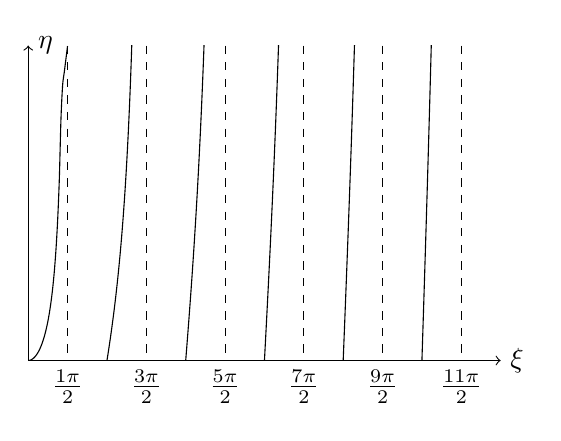
\begin{tikzpicture}
	\draw [->] (0, 0) -- (6, 0) node [right] {$\xi$};
	\draw [->] (0, 0) -- (0, 4) node [right] {$\eta$};
	\begin{scope}[yscale=2]
	\clip (0, 0) rectangle (6, 2);
	\foreach \a in {0,1,...,5} {
		\pgfmathsetmacro\b{\a + 0.499};
		\draw [domain=\a:\b] plot [smooth] (\x, {\x * min(4, tan(180*\x))});
	}
	\end{scope}
	\foreach \a in {0,1,...,5} {
		\pgfmathsetmacro\n{\a * 2 + 1};
		\draw [dashed] (\a + 0.5, 4) -- (\a + 0.5, 0) node [below] {$\frac{\pgfmathprintnumber{\n} \pi}{2}$};
	}
	\end{tikzpicture}
\end{center}
The other equation is the equation of a circle. Depending on the size of the constant $2ma^2 U/\hbar^2$, there will be a different number of points of intersections.
\begin{center}
	\begin{tikzpicture}
	\draw [->] (0, 0) -- (6, 0) node [right] {$\xi$};
	\draw [->] (0, 0) -- (0, 4) node [right] {$\eta$};
	\begin{scope}[yscale=2]
	\clip (0, 0) rectangle (6, 2);
	\foreach \a in {0,1,...,5} {
		\pgfmathsetmacro\b{\a + 0.499};
		\draw [domain=\a:\b] plot [smooth] (\x, {\x * min(4, tan(180*\x))});
	}
	\end{scope}
	\draw [mred, dashed] (2.3, 0) arc (0:90:2.3);
	\draw [mred, dashed] (1.5, 0) arc (0:90:1.5);
	\end{tikzpicture}
\end{center}

So 1 solution for \[ \frac{2ma^{2}U}{\hbar^{2}} < \pi^{2} \]

and then we have exactly $n$ even parity solutions (for $n \geq 1$).

\[ (n-1)^{2} \pi^{2}  < \frac{2ma^{2}U}{\hbar^{2}}  < n^{2} \pi^{2}  \]



We can do exactly the same thing for odd parity eigenstates\ldots on example sheet 1.


\subsection{General Properties}

Consider $ t $-indep SE for particle of mass $ m $

\[ H \psi = - \frac{\hbar^{2}}{2m} \psi''  + V(x)\psi = E \psi \]

with potential $ V(x) \to 0 $ (rapidly) as $ x \to \pm \infty $


\subsubsection{Bond State Energies}
	
	From assumption above 
	
	\[ -\frac{\hbar^{2}}{2m} \psi''  \sim E \psi \qquad x \to \pm \infty \] 
	


If $ E = \frac{\hbar^{2}k^{2}}{2m} > 0 $ then $ \psi \sim A \pm e^{ikx} + B \pm e^{-ikx} $ as $ x \to \pm \infty $.

In this case, no normalisable solution - nevertheless these solutions are of physical interest - Chapter 5. 

If $\underbrace{ E = - \frac{\hbar \kappa^{2}}{2m}}_{\kappa > 0} < 0  $ then $ \psi \sim A \pm e^{\kappa x}  + B \pm e^{- \kappa x} $ as $ x \to \pm \infty $.

2nd order ODE so 2 complex constants in general solution. 

But eqn linear and changing $ \psi \to \lambda \psi $ for any complex $ \lambda \neq 0 $ does not change physical content. Left with one complex degree of freedom

Also, for a normalisable solution we need to fix $ A_{+} = 0 $ and $ B_{-} = 0 $, imposing two conditions. Overconstrained problem $ \Rightarrow $ solutions exist only for \emph{particular} values of $ E $. 

In general, expect bound state energy levels to be \emph{quantised}. May have several solutions. 

	 \begin{center}
	%draw lines 
	\begin{tikzpicture}[yscale=1.5]
	\draw [->] (-3, 0) -- (3, 0) node [right] {$x$};
	\draw [->](0, -1.3)   -- (0, 1.3) node [above] {$V(x)$};
	\draw [domain=-3:3,samples=50, mblue] plot (\x, - {exp(-\x * \x)});
	\draw [mred, dashed] (-3, -0.7) -- (3, -0.7);
	\draw [mred, dashed] (-3, -0.6) -- (3, -0.6);
	\draw [mred, dashed] (-3, -0.9) -- (3, -0.9);
	\end{tikzpicture}
\end{center}
or none

	 \begin{center}
	%label axis x,y as x, |psi(x)|^{2}
	\begin{tikzpicture}[yscale=1.5]
	\draw [->] (-3, 0) -- (3, 0) node [right] {$x$};
	\draw [->](0, 0)  -- (0, 1.3) node [above] {$ V(x) $};
	\draw [domain=-3:3,samples=50, mblue] plot (\x, {exp(-\x * \x)});
	\end{tikzpicture}
\end{center}

Furthermore, if $V(x) \geq V_{0} $ (const) then for normalised $ \psi $ with 

\[ H \psi = E \psi \], we have 

\[ E = \langle H \rangle_{\psi} \]

\begin{align*}
& = \int_{-\infty}^{\infty}  \left(  \frac{\hbar^{2}}{2m} \psi^{*} \psi '' + \psi^{*}  V(x) \psi \right) \; \d x   \\
& = \int_{-\infty}^{\infty}  \left(  \frac{\hbar^{2}}{2m} | \psi' |^{2} + V(x) | \psi(x) |^{2} \right) \; \d x \\
& \geq 0 + \int_{-\infty}^{\infty} V_{0} | \psi(x) |^{2} \; \d x \\
& = V_{0}
\end{align*}

So in general have discrete eigenvalues with $ 0 > E > V_{0} $




Bound state is a normalisable energy eigenstate. State with lowest energy eigenvalue is called the \emph{ground state}. States with higher energy eigenvalues are often referred to as \emph{excited states}.

\subsubsection{Parity}

Consider SE with $ V(-x) = V(x) $. By changing variables $ x \to -x $ find

\[ \psi(x) \text{ eigenstate of } H \text{ with energy } E \]
\[ \iff -\psi(x) \text{ eigenstate of } H \text{ with energy } E \]

Assume $ \psi(\pm x) $ have same physical content, so that

\[ \psi(-x) = \eta \psi(x) \text{ (say)} \]

Then

\[ \psi(x) = \eta \psi(-x) = \eta^{2} \psi(x) \]
\[ \Rightarrow \eta^{2} = 1 \text{ or } \eta = \pm 1  \]

or 

\[ \psi(-x) = \pm \psi(x) \]

We say that $ \psi $ has \emph{even/odd} parity or \emph{parity} $ \eta = \pm 1 $.

The assumption above is valid for any normalisable $ \psi $ (Sheet 1 question 8).

More generally, consider linear combinations of states 

\[ \psi_{\pm}(x) = \lambda \left(   \psi(x) \pm \psi(-x ) \right) \] 

(with $ \lambda $ const) also eigenstates of $ H $ with eigenvalues $ E $

\[ \psi_{\pm}(-x) = \pm \psi_{\pm}(x) \]

so parity $ \pm 1 $ by construction. For bound states, one of these combinations vanishes. 

\subsection{Harmonic Oscillator}

Particle of mass $ m $ in a potential 



	 


	 \begin{center}
	%label axis x,y as x, |psi(x)|^{2}
	\begin{tikzpicture}[yscale=0.5]
	\draw [->] (-3, 0) -- (3, 0) node [right] {$x$};
	\draw [->](0, 0)  -- (0, 9) node [above] {$ V(x) $};
	\draw [domain=-3:3,samples=50, mblue] plot (\x, {\x *\x});
	\end{tikzpicture}
\end{center}


\[ V(x) = \frac{1}{2} m \omega^{2} x^{2} \]

($ \omega = \sqrt{k/m} $ to compare with chapter 1 and sheet 1, question 5)

Classically, in general solution

\[ x = A \cos \omega (t - t_{0}) \] 

In QM, seek all normalisable solutions of SE:
\[ H \psi = - \frac{\hbar^{2}}{2m} \psi'' + \frac{1}{2} m \omega^{2} x^{2} \psi = E \psi \]

To simplify, put

\[ y = \left( \frac{m \omega}{\hbar} \right)^{\frac{1}{2}}  \qquad \text{dimensionless}\]

SE becomes

\[ - \frac{\d^{2} \psi }{\d  y^{2} } + y^{2} \psi = \varepsilon \psi \qquad \text{ with } \varepsilon = \frac{2E}{\hbar \omega} \]


Behaviour for $ y^{2} >> \varepsilon $ suggests setting

\[ \psi = f(y) e^{- \frac{1}{2} y^{2}} \qquad \text{(wlog)} \]

and then SE holds iff

\[ \frac{\d^{2} f}{\d y^{2}} - 2y \frac{\d f}{\d y} + (\varepsilon - 1)f = 0 \]

[$ y^{2} $ term now absent, by construction]

Now seek series solution

\[ f(y) = \sum_{r\geq 0} a_{r} y^{r} \]

and substitute

\[ \sum_{r\geq 0} \left\{   (r+2)(r+1)a_{r+2} + (\varepsilon  - 1 - 2r) a_{r}    \right\} y^{r} = 0  \]


\[ \iff a_{r+2} = \frac{2r + 1 - \varepsilon}{(r+2)(r+1)} a_{r} \qquad r \geq 0 \]

This gives two linearly independent series solutions consisting of all even or all odd powers, with overall constants $ a_{0} $ and $ a_{1} $

Consider each series separately and examine behaviour of $ f(y) $ when $ y $ is large. Unless coeffs vanish,

\begin{center}
	\begin{tabular}{rlll}
		for even series & $a_{2p} / a_{2p - 2} $ & $\sim \frac{1}{p}$ & $ \quad p \to \infty $\\
		for odd series & $a_{2p+1} / a_{2p - 1} $ & $\sim \frac{1}{p}$ & $ \quad  p \to \infty $
	\end{tabular}
\end{center}

which matches behaviour of $ y^{\alpha} e^{y^{2}} $ for some $ \infty $

eg

\[ \sum \frac{1}{p!} y^{2p}, \quad \sum \frac{1}{p!} y^{2p + 1}  \]

Such behaviour for $ f \Rightarrow \psi \sim \text{ (poly in y) }e^{\frac{1}{2}y^{2}}  $ not normalisable

Hence $ \psi $ is a normalisable solution iff series for $ f $ terminates, giving a polynomial. This happens iff

\[ \varepsilon = 2n + 1 \qquad \text{ for } n = 0,1,2,\cdots \]

Solutions:

\[ \begin{cases}  a_{r+2} = \frac{2r - 2n}{(r+2)(r+1)} a_{r} & \text{ if } n \text{ even} \\ a_{r} = 0 & \text{ if } n \text{ odd}\end{cases} \]

Solutions

\[ f(y) = h_{n}(y) \text{ poly of degree } n \text{ with} \]

\[ h_{n}(-y) = (-1)^{n} h_{n}(y) \]

eg.


\begin{align*}
h_{0}(y) & = a_{0}  \qquad \varepsilon = 1\\
h_{1}(y) & = a_{1} y \qquad \varepsilon = 3\\
h_{2}(y) & = a_{0} (1 - 2y^{2}) \qquad \varepsilon = 5\\
h_{3}(y) & = a_{1} a_{1} (y - \frac{2}{3} y^{3}) \qquad \varepsilon = 7\\
\end{align*}

The ODE for $ f $ is called \emph{Hermite's equation}, and solutions are \emph{Hermite polynomials}

Restoring constants- harmonic oscillator eigenvalues and eigenfunction are

\[ E_{n} = \hbar \omega  (n + \frac{1}{2}) \quad \text{ and } \quad \psi_{n}(x) = h_{n} \left(  \left(\frac{m \omega}{\hbar}   \right)^{\frac{1}{2}}  x \right)  e^{-\frac{1}{2} \left( \frac{m \omega}{\hbar} \right) x^{2} }     \]

for $ n = 0,1,2,\cdots $

There are many important applications of these results.

\begin{enumerate}
	\item Any smooth potential can be approximated by an oscillator near a minimum $ x_{0} $:
	
	\[ V(x) \simeq V(x_{0}) + \frac{1}{2} V''(x_{0}) (x - x_{0})^{2} + \cdots \]
	
	frequency
	
	\[ \omega = \sqrt{V''(x_{0}) / m} \]
	
	\item Systems with many degrees of freedom e.g. crystals can be analysed by reducing to \emph{normal modes} of oscillation
	
	\item Quantised EM fields: one oscillator for each mode of vibration with $ n $th state of this oscillator interpreted as $ n $ photons with $ E_{n} - E_{0} = n \hbar \omega $
	
	Underlies full explaination (QFT) of wave/particle duality
	
\end{enumerate}


\section{Expectation and Uncetainty}

\subsection{Hermitian Operators}

Recall definition:

\[ (\phi,\psi)  = \int_{-\infty}^{\infty} \phi(x)^{*} \; \d x \]

which obeys

\[ (\phi,\alpha \psi) = \alpha (\phi,\psi) = (\alpha^{*} \phi,\psi ) \]

and

\[ (\phi,\psi) = (\psi,\phi)^{*} \]

Regrading this as an inner product on wavefns, define the norm $ | | \psi | | $ of a wavefn $ \psi $ by

\[ | | \psi | |^{2} = (\psi,\psi) = \int_{-\infty}^{\infty} | \psi(x) |^{2} \; \d x \]

so $ \psi $ normalised iff $ | | \psi | | =1 $.

An operator $ Q $ is \emph{hermitian} if

\[ (\psi, Q \psi) = (Q \psi, \psi) \qquad \forall \text{ normalisiable } \psi, \phi \]

or 

\[ \int_{-\infty}^{\infty} \phi^{*} Q \psi \; \d x = \int_{-\infty}^{\infty} (Q \phi)^{*} \psi \; \d x \]

This implies 
\[ (\psi, Q \psi) = (Q \psi, \psi) = (\psi, Q \psi)^{*} \]

or

\[ \langle Q \rangle_{\psi} =  \langle Q \rangle_{\psi}^{*}\]

The operators $ \hat{x} $, $ \hat{p} $ and $ H  = \frac{\hat{p}^{2}}{2m} + V(\hat{x}) $ are hermitian for $ V $ real.

\begin{proof}
	\begin{align*}
	& (\phi, \hat{x} \psi ) = (\hat{x}\phi, \psi ) \\
	\iff &   \int_{-\infty}^{\infty} \phi(x)^{*} (x \psi(x)) \; \d x \\
	\iff &  \int_{-\infty}^{\infty} (x \psi(x))^{*} \phi(x) \; \d x
	\end{align*}
	
	$ x $ real
	
	
	\begin{align*}
	& = (\phi, \hat{p} \psi ) = (\hat{p}\phi, \psi ) \\\iff &   \int_{-\infty}^{\infty} \phi^{*} (-i \hbar \psi') \; \d x \\
	\iff &  \int_{-\infty}^{\infty} (-i\hbar \phi')^{*} \psi(x) \; \d x
	\end{align*}
	
	by parts, since $  - i \hbar \left[  \phi^{*} \psi \right]_{-\infty}^{\infty}  $
	
	To show 
	
	\[ (\phi, H \psi) = (H \phi,\psi) \]
	
	consider k.e and p.e terms separately
	
	ke
	%table
	
	$ (\phi, \psi'') = - (\phi',\psi') = (\phi'',\psi) $
	
	pe
	$ (\phi,V(\hat{x})\psi  )  = (V(\hat{x})\phi, \psi )  $ since $ V $ real.
	
	This gives better understanding why $ <\hat{x}>, <\hat{p}> $ and $ <H>$ are real	
\end{proof}
	
\subsection{Ehrenfest's Theorem - QM is like classical mechanics}
	
Consider normalised $ \Psi(x,t) $ satisfying time-dep SE

\[ i \hbar \dot{\Psi} = H \Psi = \left(  \frac{1}{2m} \hat{p}^{2} + V (\hat{x}) \right) \Psi = - \frac{\hbar^{2}}{2m} \Psi'' + V(x) \Psi  \]

The expectation values $ <\hat{x}>_{\Psi} = (\Psi, \hat{x} \Psi) $ and $  <\hat{p}>_{\Psi} = (\Psi, \hat{p} \Psi) $ depend on $ t $ through $ \Psi $

Ehrenfest's Thm states

\[ \frac{\d }{\d t}  <\hat{x}>_{\Psi} = \frac{1}{m} <\hat{p}>_{\Psi} \]

and

\[ \frac{\d }{\d t}  <\hat{p}>_{\Psi} = - <V'(\hat{x})>_{\Psi} \]
	
quantum counterparts of classical eqns of motion.

\begin{proof}
	\[ \frac{\d }{\d t} <\hat{x}>_{\Psi} = (\dot{\Psi}, \hat{x} \Psi ) + (\Psi, \hat{x} \dot{\Psi} ) \]
	
	\[  = (\frac{1}{i \hbar}  H \Psi, \hat{x} \Psi  )   + (\Psi,  \hat{x} \frac{1}{i \hbar}  H \Psi   ) \qquad \text{SE} \]
	
	\[ = \frac{1}{i \hbar}(  H \Psi, \hat{x} \Psi  )   + \frac{1}{i \hbar}(\Psi,  \hat{x} H \Psi   ) \]
	
	\[ = \frac{1}{i \hbar}( \Psi, H \hat{x} \Psi  )   + \frac{1}{i \hbar}(\Psi,  \hat{x} H \Psi   ) \]
	
		\[ = \frac{1}{i \hbar}( \Psi, (\hat{x} H - H \hat{x}  ) \Psi   ) \]
	
	Now
	
	\begin{align*}
	(\hat{x} H - H \hat{x}  ) \Psi & = - \frac{\hbar^{2}}{2m}(x \Psi'' - (x \Psi)'') + (xV - Vx) \Psi  \\
	& = - \frac{\hbar^{2}}{2m} \Psi' = \frac{i\hbar}{m} \hat{p} \Psi \quad \text{ as req}
	\end{align*}
	
	
	Similarly, 
	
	\begin{align*}
	\frac{\d }{\d t}  <\hat{p}>  & =  (\dot{\Psi}, \hat{p} \Psi )  + (\Psi, \hat{p}  \dot{\Psi} )  \\
	& = (+ \frac{1}{i \hbar}H \Psi, \hat{p} \Psi  ) + (\Psi, \hat{p} \frac{1}{i \hbar } H \Psi  ) \\
	& = \frac{1}{i \hbar} (\Psi, (\hat{p}H - H\hat{p})\Psi  ) 
	\end{align*}
	
	But
	
	\begin{align*}
	(\hat{p}H - H\hat{p})\Psi& = - i \hbar \left( - \frac{\hbar^{2}}{2m} \right) \left(  (\psi'')' - (\psi')'' \right)   \\
	& = - i \hbar \left(  (V(x)\Psi)' - V(x)  \Psi' \right) \\
	& = - i \hbar V'(x) \Psi \qquad \text{ as req}
	\end{align*}
	
	In each case it is the \emph{commutator} that appears:
	
	\[ \hat{x} H - H \hat{x}  \text{ and } \hat{p}H - H\hat{p})\Psi\]
	
	
	
\end{proof}

 
\subsection{Heisenberg's Uncertainty Relation - QM is NOT like classical mechanics}





Statement: If $ \psi $ is any normalised state (at fixed time) define the \emph{uncertainty} $ m $ position and momentum $ (\Delta x)_{\psi} $ and $ (\Delta p)_{\psi} $ by

\[ (\Delta x)_{\psi}^{2} = \langle (\hat{x}  - \langle \hat{x} \rangle_{\psi} )^{2} \rangle_{\psi} = \langle \hat{x}^{2} \rangle_{\psi} - \langle \hat{x} \rangle_{\psi}^{2} \]

\[ (\Delta p)_{\psi}^{2} = \langle (\hat{p}  - \langle \hat{p} \rangle_{\psi} )^{2} \rangle_{\psi} = \langle \hat{p}^{2} \rangle_{\psi} - \langle \hat{p} \rangle_{\psi}^{2} \]

These quantify the `spread' of possible results. Heisenberg's Uncertainty Relation or Principle, states

\[ (\Delta x)_{\psi} (\Delta p)_{\psi} \geq \frac{\hbar}{2} \]

Interpretation: we can never reduce combined uncertainty in position and momentum below this threshold. 


Note $ X = \hat{x} - \alpha $ and $ P = \hat{p} - \beta $ both hermitian for any real constants $ \alpha $ and $ \beta $. This implies 

\begin{align*}
(\psi, X^{2}\psi)& = (X\psi, X\psi)  = | | X \psi | |^{2} \geq 0
\end{align*}

and 

\begin{align*}
(\psi, P^{2}\psi)& = (P\psi, P\psi)  = | | P \psi | |^{2} \geq 0
\end{align*}

Choosing $ \alpha = <\hat{x}>_{\psi} $ and $ \beta = <\hat{p}>_{\psi} $ we deduce that $ (\Delta x)_{\psi}^{2}  $ and $ (\Delta p)_{\psi}^{2} $ are indeed real and positive

\begin{eg}
	Gaussian \[ \psi(x) = \left( \frac{1}{\alpha \pi} \right) ^{\frac{1}{4}} e^{- \frac{x^{2}}{2 \alpha}} \]
	
	has $ \langle \hat{x} \rangle_{\psi} = \langle \hat{p} \rangle_{\psi} = 0$

and $ (\Delta x)_{\psi}^{2}  = \frac{\alpha}{2} $ and $ (\Delta p)_{\psi}^{2} = - \frac{\hbar^{2}}{2 \alpha}$

So 

\[ (\Delta x)_{\psi} (\Delta p)_{\psi} = \frac{\hbar}{2} \]

minimum allowed by Heisenberg.

Furthermore, this is ground state of the Harmonic oscillator for 

\[ \alpha = \frac{\hbar}{m \omega} \]

Classically, lowest energy from oscillator is when $ x = p = 0 $. 

%particle sitting at bottom of potential doing nothing

In QM can't have exact values for $ x $ and $ p $ in this way, and minimum energy $ E_{0} = \frac{1}{2} \hbar \omega $ consistent with this. 


Particle of mass $ m $ in a potential 


\begin{center}
	%label axis x,y as x, |psi(x)|^{2}
	\begin{tikzpicture}[yscale=0.5]
	\draw [->] (-3, 0) -- (3, 0) node [right] {$x$};
	\draw [->, mred, dashed] (-3, 1) -- (3, 1) node [right] {$\frac{1}{2} \hbar \omega$};
	\draw [->](0, 0)  -- (0, 9) node [above] {$ V(x) $};
	\draw [domain=-3:3,samples=50, mblue] plot (\x, {\x *\x});
	\end{tikzpicture}
\end{center}


\end{eg}



(a)

Statement:

\[ (\Delta x)_{\psi} (\Delta p)_{\psi} \geq \frac{\hbar}{2} \]

for any normalisable state $ \psi $

\[ (\Delta x)_{\psi}^{2} = (X\psi, X \psi) \]

\[ (\Delta p)_{\psi}^{2} = (P \psi, P \psi) \]

\[ X = \hat{x} - < \hat{x} >_{\psi} \]
\[ P = \hat{p} - < \hat{p} >_{\psi} \]



(b)
\begin{proof}
	The uncertainty relation follows from the \emph{canonical commutation relation}



\[ [\hat{x} ,\hat{p} ] : = \hat{x}\hat{p} - \hat{p} \hat{x} = i \hbar \]

This holds since

\begin{align*}
(\hat{x}\hat{p} - \hat{p} \hat{x}) \psi & =  x ( - i \hbar \psi') + i \hbar (x \psi)' \\
& = i \hbar \psi
\end{align*}

as required.

For any normalised $ \psi $, consider 

\begin{align*}
| |   (X + i \lambda P) \psi  | |^{2}  & =  (  (X + i \lambda P)\psi, (X + i \lambda P )\psi) \\
& = (X\psi, X \psi) + i \lambda (  X \psi, P \psi) - i \lambda (P \psi, X \psi) + \lambda^{2} (P \psi, P \psi) 
\geq 0 \text{ for any real } \lambda
\end{align*}

But then

\[ (\Delta x)_{\psi}^{2} + i \lambda (X \psi, P \psi) - i \lambda(P \psi, X \psi) + \lambda^{2}  (\Delta p)_{\psi}^{2} \geq 0  \]

and

\begin{align*}
(X \psi, P \psi) - (P \psi, X \psi)  & =  (\psi, X P \psi) - (\psi) \text{ since } X \text{ and } P \text{ are Hermitian}  \\
& = (\psi, [X,P]\psi) \\
& = (\psi, i \hbar \psi) \\
& = i \hbar
\end{align*}

Since $ [X,P] = [\hat{x},\hat{p}] = i \hbar $

Hence

\[ (\Delta x)_{\psi}^{2} + \lambda^{2} (\Delta p)_{\psi}^{2} - \lambda \hbar \geq 0  \text{ for any real } \lambda \]

In fact, by inspection, $ (\Delta x)_{\psi}^{2} $ and $ (\Delta p)_{\psi}^{2} > 0 $.

Choosing $ \lambda = (\Delta x)_{\psi} / (\Delta p)_{\psi} $ then gives the desired result.

\end{proof}

\section{Scattering in One Dimension}

Many interesting physical processes involve a particle fired at a target and being \emph{scattered} (What is the probability of scattering a particular direction?)

In one dimension, we can consider an incident wavepacket $ \Psi_{\text{inc}} $ interacting with a potential which then evolves into a reflected and a transmitted wavepacket. 

``Early times''
	 \begin{center}
	% \draw [ ->](0, 0) -- (0,1.3) node[above] {$| \psi(x) |^{2}$
	%dashed vertical line going through the second wave, label with x_{0}
	\begin{tikzpicture}[xscale=0.75, yscale=1.5]
	\draw [ ->](-9, 0) -- (3, 0) node[right] {$x$};
	\draw [ ->](0, 0) -- (0,1.3) node[above] {$ V(x) $};
	\draw [dashed] (-6, -0.5) node[below] {$ \Psi_{\text{inc}}  $} -- (-6,1.3) ;
	\draw [->] (-6, 1) -- (-5, 1);
	\draw [domain=-9:3,samples=80, mblue] plot (\x, {exp(-\x * \x) + exp(-(\x + 6)^2/4)});
	\end{tikzpicture}
\end{center}
``Late times''
\begin{center}
	% \draw [ ->](0, 0) -- (0,1.3) node[above] {$| \psi(x) |^{2}$
	%dashed vertical line going through the second wave, label with x_{0}
	\begin{tikzpicture}[xscale=0.75, yscale=1.5]
	\draw [ ->](-9, 0) -- (9, 0) node[right] {$x$};
	\draw [ ->](0, 0) -- (0,1.3) node[above] {$ V(x) $};
	\draw [dashed] (-6, -0.5) node[below] {$ \Psi_{\text{inc}}  $} -- (-6,1.3) ;
	\draw [->] (-6, 1) -- (-7, 1);
	\draw [->] (6, 1) -- (7, 1);
	\draw [dashed] (6, -0.5) node[below] {$ \Psi_{\text{tr}}  $} -- (6,1.3) ;
	\draw [domain=-9:9,samples=80, mblue] plot (\x, {exp(-\x * \x) + exp(-(\x + 6)^2/4) + exp(-(\x - 6)^2/4)});
	\end{tikzpicture}
\end{center}



Solving the t-dep SE for such a problem is difficult. Seek instead a stationary state solution

\subsection{Momentum Eigenstates and Particle Beams}

Recall eigenstates of $ \hat{p} = - i \hbar \frac{\partial }{\partial x} $ are 

\[ \psi = C e^{i k x} \text{ with } \hat{p} \psi = p \psi, \text{ eval } p = \hbar k \]

and these are \emph{not} normalisable on $ - \infty < x < \infty $.

Could impose \emph{periodic boundary conditions} $ \phi(x + l) = \phi(x) $ and restrict to an interval or ``box'' $ - \frac{l}{2} \leq x \leq \frac{l}{2} $. Then eigenstates can be normalised and we can talk $ l \to \infty $ after completing calculations.

A convenient alternative is to allow \emph{non-normalisable} but bounded wavefunctions. For $ V = 0 $:

\[ \Psi(x,t) = C e^{ikx} e^{-iEt/\hbar} \]

stationary state with $ E = \hbar^{2} k^{2} / 2m $

Interpretation:

\begin{enumerate}
	\item bean of particles, each with momentum and $ p = \hbar k $ and energy $ E = - \hbar^{2} k^{2} / 2m $.
	\item average particle density (number per unit length) is $ | C |^{2} $.
	\item \emph{Flux} on particles is given by the current 
	
	\begin{align*}
	J & = - \frac{i \hbar}{2m}  (  \Psi^{*} \Psi' - \Psi'^{*} \Psi ) \quad \text{ (number passing a given point per unit time) } \\
	& = | C |^{2}  \frac{\hbar k}{m}  \quad \text{ (number density times velocity ) } \end{align*}
	Moreover, superposition of beams 
	
	\[ \Psi(x,t) = (  C_{+} e^{ikx}   + C_{-}  e^{-ikx}   ) e^{-iEt/\hbar}  \]
	
	$ p = \hbar k $, $ p = -hbar k $ same energy.
	
	\begin{align*}
	\Rightarrow J(x,t) & = | C_{+} |^{2} \frac{\hbar k}{m} + | C_{-} |^{2}  \left(  - \frac{\hbar k}{m} \right) \qquad (\text{cross terms cancel})   \\
	\end{align*}
	
	\item Probabilities are calculated by comparing fluxes.
	
\end{enumerate}

To justify assumptions and interpretations using beams, we can refer back to one-particle description in a box.

\subsection{Potential Step}


Consider solution $ \Psi(x,t) = \phi(x) e^{-iEt/\hbar} $ to SE with potential 

\[ V(x)  = \begin{cases} 0  & \text{ if } x \leq 0 \\   u & \text{ if } x > 0 \end{cases}\]


\begin{center}
	% \draw [ ->](0, 0) -- (0,1.3) node[above] {$| \psi(x) |^{2}$
	%dashed vertical line going through the second wave, label with x_{0}
	\begin{tikzpicture}[xscale=0.75, yscale=1.5]
	\draw [ ->](-3, 0) -- (3, 0) node[right] {$x$};
	\draw [ ->](0, 0) -- (0,1.3) node[above] {$ V(x) $};
	\draw [-,mblue] (-3,0) -- (0,0); 
	\draw [-,mblue] (0,1) -- (3,1)  node [right] {$ u > 0 $}  ; 
	\end{tikzpicture}
\end{center}
	
	$ \phi $ satifies t dep SE
	
	$ \phi,\phi' $ continuous at $ x = 0 $
	
	Current
	
	
	\[ J = - \frac{i \hbar}{2m}  ( \psi^{*}  \psi'   - \psi'^{*} \psi ) \]
	
	
\begin{enumerate}
	\item $ E > U $
	
	Set 
	
	\[ E = \frac{\hbar^{2} k^{2}}{2m}  \qquad E - U = \frac{\hbar^{2} l^{2}}{2m} \quad (k,l > 0) \]
	
	SE becomes
	
	\[ \phi'' + k^{2} \phi = 0 \qquad  \phi'' + l^{2} \phi = 0 \]
	
	\[ x < 0 \qquad x > 0 \]
	
	\[ \Rightarrow \phi = I e^{ikx} + R e^{-ikx}  \qquad \phi = T e^{ilx}   \]
	
	( No $ e^{-ilx} $ term $ \iff $ no particles sent from right )
	
	Match at $ x = 0 $
	
	\[ \phi \text{ continuous } I + R = T \]
	\[ \phi' \text{ continuous } ik I - i k R = i l T \]
	
	
	\[ \Rightarrow  R = \frac{k-l}{k+l} I \qquad T = \frac{2k}{k+l}I \]
	
	Current
	
	\begin{align*}
	J & = J_{\text{inc}} + J_{\text{ref}} \\
	& = (  | I |^{2} - | R |^{2}  ) \frac{\hbar k}{m}  \qquad (x < 0)
	\end{align*}
	
	
	
	and
	
	\begin{align*}
	J & = | T |^{2}  \frac{\hbar l}{m} \qquad (x > 0) \\
	\end{align*}	
	
	
	Probability of reflection 
	
	\[ P_{\text{ref}} = \frac{| J_{\text{ref}} |}{ | J_{\text{inc}} |} = \frac{|R|^{2}}{| I |^{2}} = \left(  \frac{k-l}{k+l} \right)^{2}  \]
	
	Probability of transmission
	
	\[ P_{\text{tr}} = \frac{| J_{\text{tr}} |}{ | J_{\text{inc}} |} = \frac{| T |^{2}}{| I |^{2}} \frac{l}{k}  = \frac{4kl}{(k+1)^{2}}  \]	
		
		
	\end{enumerate}










  \end{document}